% ============================================================================
% SIH 26171 - On-device Visual Perception for Light-weight Browser Agents
% Prototype Report (standalone PDF, generated from the report Markdown)
% Compile: pdflatex (run twice for TOC)  |  also works with xelatex/lualatex
% ============================================================================
\documentclass[11pt,a4paper]{article}

\usepackage[margin=2.4cm]{geometry}
\usepackage[T1]{fontenc}
\usepackage[utf8]{inputenc}
\usepackage{lmodern}
\usepackage{microtype}
\usepackage{xcolor}
\usepackage{booktabs}
\usepackage{tabularx}
\usepackage{ragged2e}
\usepackage{array}
\usepackage{enumitem}
\usepackage{float}
\usepackage[font=small,labelfont=bf]{caption}
\usepackage{titlesec}
\usepackage{fancyhdr}
\usepackage{amsmath}
\usepackage{tikz}
\usetikzlibrary{arrows.meta,positioning,calc}
\usepackage[hidelinks]{hyperref}

% ---------------------------------------------------------------------------
% Brand colors
% ---------------------------------------------------------------------------
\definecolor{primary}{RGB}{40,53,147}   % deep indigo
\definecolor{secondary}{RGB}{13,110,253}% blue
\definecolor{accent}{RGB}{182,40,53}    % deep red (privacy / redaction theme)
\definecolor{codebg}{RGB}{245,245,248}
\definecolor{good}{RGB}{21,128,61}      % green (PASS)
\definecolor{bad}{RGB}{182,40,53}       % red

% ---------------------------------------------------------------------------
% Helpers
% ---------------------------------------------------------------------------
\newcommand{\code}[1]{\texttt{#1}}
\newcommand{\arw}{$\rightarrow$}
\newcommand{\rar}{\rightarrow}

\titleformat{\section}{\Large\bfseries\color{primary}}{\thesection}{0.7em}{}
\titleformat{\subsection}{\large\bfseries\color{secondary}}{\thesubsection}{0.6em}{}
\titlespacing*{\section}{0pt}{14pt}{6pt}
\titlespacing*{\subsection}{0pt}{10pt}{4pt}

\fancypagestyle{plain}{%
  \fancyhf{}
  \fancyhead[L]{\footnotesize\color{black!60}SIH 26171 --- Prototype Report}
  \fancyhead[R]{\footnotesize\color{black!60}\thepage}
  \renewcommand{\headrulewidth}{0.3pt}
}
\pagestyle{plain}

\setlist{nosep, leftmargin=1.4em}
\setlength{\parskip}{4pt}
\renewcommand{\arraystretch}{1.2}

\hypersetup{
  pdftitle={SIH 26171 - On-device Visual Perception for Light-weight Browser Agents (Prototype Report)},
  pdfauthor={SIH 26171 Team},
  pdfsubject={Privacy-preserving browser agent prototype report},
}

% ---------------------------------------------------------------------------
% Document
% ---------------------------------------------------------------------------
\begin{document}

% ============================================================================
% TITLE BLOCK
% ============================================================================
\begin{center}
  {\color{primary}\rule{\linewidth}{1.5pt}}\\[6pt]
  {\LARGE\bfseries\color{primary} On-device Visual Perception for\\[2pt] Light-weight Browser Agents}\\[8pt]
  {\large SIH 26171 --- Prototype Report}\\[6pt]
  {\normalsize Smart India Hackathon 2026 ~~$\cdot$~~ Research track}\\[10pt]
  {\color{primary}\rule{\linewidth}{0.6pt}}
\end{center}

\begin{center}
\renewcommand{\arraystretch}{1.5}
\begin{tabular}{@{}ll@{}}
  \textbf{Problem statement} & Build a privacy-preserving browser agent that understands a web\\
  & page \emph{on the user's own device}, redacts all personal data \emph{before}\\
  & anything leaves the machine, and only then asks a local language\\
  & model to decide the next action --- enabling a user to automate\\
  & browsing tasks (form-filling, searches, navigation, reading dashboards)\\
  & without ever shipping screenshots full of Aadhaar numbers, PAN cards,\\
  & bank details, or faces to a remote server.\\[2pt]
  \textbf{Approach in one line} & Sanitise on-device ($\rightarrow$ the VLM never sees raw PII), ground\\
  & every action by element ID, decide with a local Qwen2.5-VL, adapt\\
  & with a structurally-vetoing recovery planner.\\
\end{tabular}
\end{center}

\vspace{4pt}

% ============================================================================
% 1. SCORING CRITERIA
% ============================================================================
\section{Scoring Criteria}

The judges weight five criteria. Every number in this report maps to one of them:

\begin{table}[H]
\centering
\small
\begin{tabularx}{\textwidth}{>{\raggedright\arraybackslash}p{3.6cm} c X}
\toprule
\textbf{Criterion} & \textbf{Weight} & \textbf{What judges look for}\\
\midrule
Visual-context accuracy & \textbf{25\%} & Can the agent complete real browsing tasks? Does the VLM correctly interpret the page and choose the right action?\\
\addlinespace
PII detection recall / precision & 20\% & Does the system catch all personal data (recall) without flagging non-PII (precision)? Measured pixel-level on ground-truth-labelled test pages.\\
\addlinespace
Redaction precision & 20\% & Of the pixels the system redacted, how many were actually PII? High precision = minimal over-redaction = the VLM still sees enough context to act.\\
\addlinespace
Client resource utilization & 20\% & How heavy is the on-device work per step? Model size, bundled assets, vision latency, OCR-gate cost --- all measured, all local.\\
\addlinespace
End-to-end latency & 15\% & How fast is one full step (capture \arw\ sanitise \arw\ VLM \arw\ execute)? Target: $<5$~s/step on a judge-class GPU.\\
\bottomrule
\end{tabularx}
\end{table}

\subsection*{How the metrics are measured}
All accuracy metrics are computed on \textbf{rasterised redaction masks} --- the union of predicted redaction bounding boxes versus the union of ground-truth boxes, clipped to the captured viewport. This is a set-based measure (not per-element), so recall and precision are bounded by 1 by construction. Ground truth is encoded as \code{data-gt} attributes on every PII element in the test pages (including AI-generated faces and PII drawn into \code{canvas} elements). An automated Playwright harness loads each page, runs the sanitiser, computes pixel overlap, and writes results to JSON --- fully reproducible, zero manual scoring.

% ============================================================================
% 2. HOW THE PROTOTYPE WORKS
% ============================================================================
\section{How the Prototype Works}

The prototype is an \textbf{end-to-end autonomous browser agent that runs a closed loop on the user's own machine}. A screenshot and a structured DOM snapshot are captured, \textbf{sanitised on-device so no personal data ever leaves}, and only the redacted payload is sent to a \textbf{local} vision-language model (VLM), which returns one JSON action to execute back in the tab. The loop repeats until the task is done.

\begin{figure}[H]
\centering
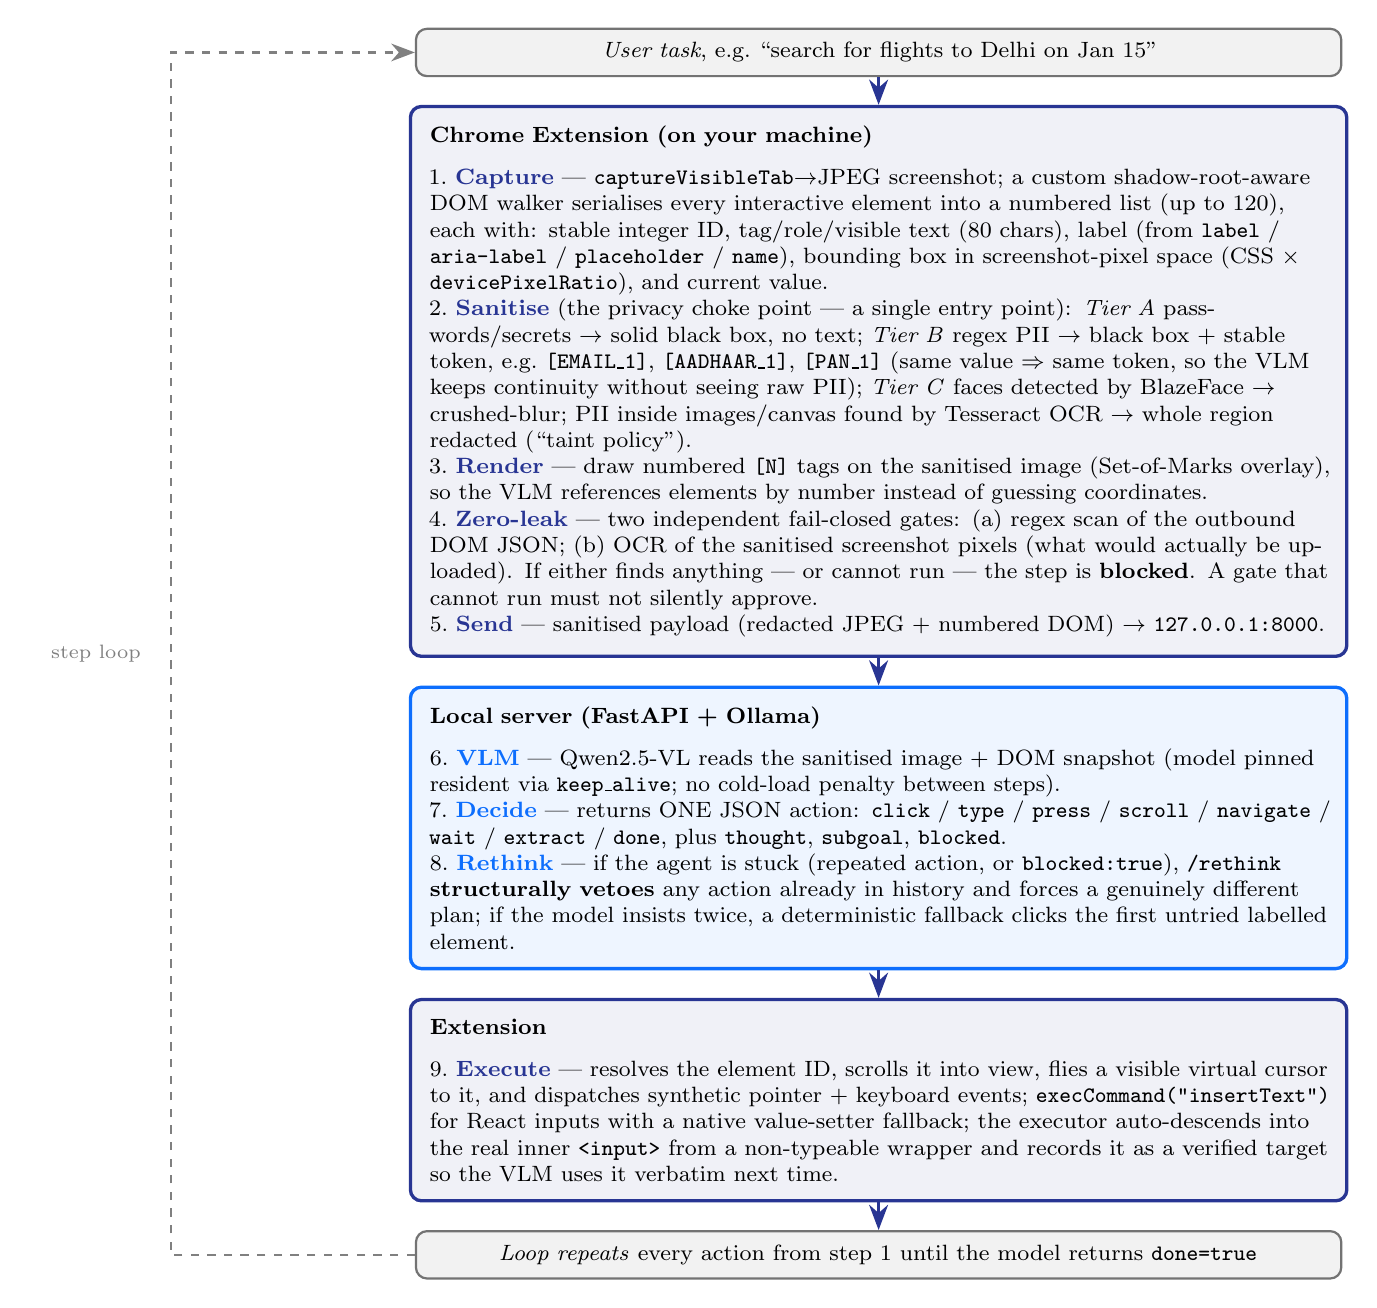
\begin{tikzpicture}[
  ext/.style={draw=primary, very thick, rounded corners=4pt, fill=primary!7, text width=11.4cm, align=left, font=\footnotesize, inner sep=7pt},
  srv/.style={draw=secondary, very thick, rounded corners=4pt, fill=secondary!7, text width=11.4cm, align=left, font=\footnotesize, inner sep=7pt},
  act/.style={draw=black!55, thick, rounded corners=4pt, fill=black!5, text width=11.4cm, align=center, font=\footnotesize, inner sep=5pt},
  arr/.style={-{Stealth[length=3.2mm]}, very thick, color=primary},
  ret/.style={-{Stealth[length=3mm]}, dashed, thick, gray},
]
\node[act] (task) {\emph{User task}, e.g.\ ``search for flights to Delhi on Jan 15''};

\node[ext, below=3.5mm of task] (ext) {%
  \textbf{Chrome Extension (on your machine)}\\[2mm]
  1.~{\color{primary}\textbf{Capture}} --- \code{captureVisibleTab}$\rightarrow$JPEG screenshot; a custom shadow-root-aware DOM walker serialises every interactive element into a numbered list (up to 120), each with: stable integer ID, tag/role/visible text (80~chars), label (from \code{label} / \code{aria-label} / \code{placeholder} / \code{name}), bounding box in screenshot-pixel space (CSS $\times$ \code{devicePixelRatio}), and current value.\\
  2.~{\color{primary}\textbf{Sanitise}} (the privacy choke point --- a single entry point):
  \emph{Tier A} passwords/secrets $\rightarrow$ solid black box, no text;
  \emph{Tier B} regex PII $\rightarrow$ black box + stable token, e.g.\ \code{[EMAIL\_1]}, \code{[AADHAAR\_1]}, \code{[PAN\_1]} (same value $\Rightarrow$ same token, so the VLM keeps continuity without seeing raw PII);
  \emph{Tier C} faces detected by BlazeFace $\rightarrow$ crushed-blur; PII inside images/canvas found by Tesseract OCR $\rightarrow$ whole region redacted (``taint policy'').\\
  3.~{\color{primary}\textbf{Render}} --- draw numbered \code{[N]} tags on the sanitised image (Set-of-Marks overlay), so the VLM references elements by number instead of guessing coordinates.\\
  4.~{\color{primary}\textbf{Zero-leak}} --- two independent fail-closed gates: (a)~regex scan of the outbound DOM JSON; (b)~OCR of the sanitised screenshot pixels (what would actually be uploaded). If either finds anything --- or cannot run --- the step is \textbf{blocked}. A gate that cannot run must not silently approve.\\
  5.~{\color{primary}\textbf{Send}} --- sanitised payload (redacted JPEG + numbered DOM) $\rightarrow$ \code{127.0.0.1:8000}.
};

\node[srv, below=3.5mm of ext] (srv) {%
  \textbf{Local server (FastAPI + Ollama)}\\[2mm]
  6.~{\color{secondary}\textbf{VLM}} --- Qwen2.5-VL reads the sanitised image + DOM snapshot (model pinned resident via \code{keep\_alive}; no cold-load penalty between steps).\\
  7.~{\color{secondary}\textbf{Decide}} --- returns ONE JSON action: \code{click} / \code{type} / \code{press} / \code{scroll} / \code{navigate} / \code{wait} / \code{extract} / \code{done}, plus \code{thought}, \code{subgoal}, \code{blocked}.\\
  8.~{\color{secondary}\textbf{Rethink}} --- if the agent is stuck (repeated action, or \code{blocked:true}), \code{/rethink} \textbf{structurally vetoes} any action already in history and forces a genuinely different plan; if the model insists twice, a deterministic fallback clicks the first untried labelled element.
};

\node[ext, below=3.5mm of srv] (exec) {%
  \textbf{Extension}\\[2mm]
  9.~{\color{primary}\textbf{Execute}} --- resolves the element ID, scrolls it into view, flies a visible virtual cursor to it, and dispatches synthetic pointer + keyboard events; \code{execCommand("insertText")} for React inputs with a native value-setter fallback; the executor auto-descends into the real inner \code{<input>} from a non-typeable wrapper and records it as a verified target so the VLM uses it verbatim next time.
};

\node[act, below=3.5mm of exec] (done) {\emph{Loop repeats} every action from step 1 until the model returns \code{done=true}};

\draw[arr] (task) -- (ext);
\draw[arr] (ext) -- (srv);
\draw[arr] (srv) -- (exec);
\draw[arr] (exec) -- (done);

\draw[ret] (done.west) -- ++(-3.1,0) |- (task.west);
\node[gray, font=\scriptsize, text width=1.5cm, align=center] at ([xshift=-4.05cm]$(done.west)!0.5!(task.west)$) {step loop};

\end{tikzpicture}
\caption{End-to-end closed-loop architecture. Only the redacted image and numbered DOM ever leave the extension; only a JSON action ever comes back.}
\end{figure}

\subsection{The components}

\subsubsection*{Chrome Extension (WXT framework, TypeScript, Chrome MV3) --- four entrypoints}

\begin{table}[H]
\centering
\small
\begin{tabularx}{\textwidth}{>{\raggedright\arraybackslash}p{3.6cm} X}
\toprule
\textbf{Entrypoint} & \textbf{Role}\\
\midrule
\code{background.ts} & \textbf{Orchestrator.} Drives the loop: \code{captureVisibleTab}$\rar$sanitise$\rar$zero-leak gate$\rar$\code{POST /act}$\rar$execute in tab. Handles throttled step scheduling, stuck detection, and recovery routing to \code{/rethink}.\\
\addlinespace
\code{content-scripts/} & \textbf{Executor + DOM serializer.} The executor converts JSON actions into real browser events (synthetic pointer/keyboard with a visible virtual cursor). The DOM walker serialises the page into a compact, numbered snapshot (shadow-root aware, capped at 120 elements).\\
\addlinespace
\code{sidepanel/main.ts} & \textbf{Control UI.} Task input, ``Run one step'', capture preview, live activity log, and a live ``thinking'' readout of the VLM's tokens via SSE streaming.\\
\addlinespace
\code{offscreen/main.ts} & \textbf{On-device vision host} (offscreen document). MediaPipe BlazeFace face detection and Tesseract OCR run here, in a DOM context, with all weights bundled locally.\\
\bottomrule
\end{tabularx}
\end{table}

\subsubsection*{Server, VLM, test site, benchmarks}
\begin{itemize}
  \item \textbf{Server} (FastAPI, Python) --- a thin app over a local Ollama instance via the OpenAI-compatible API. Endpoints: \code{/health}, \code{/warm}, \code{/act}, \code{/act/stream}, \code{/rethink}, \code{/rethink/stream}, \code{/models}. It builds the VLM prompt (image + DOM), calls the model, and returns a validated action response. It also mounts the test site as static files.
  \item \textbf{VLM} --- \textbf{Qwen2.5-VL 3b / 7b} running locally in Ollama. Ollama pins the model resident (\code{keep\_alive:-1}), so the 20--60~s cold-load cost is paid once, not every step.
  \item \textbf{Test site} --- seven ground-truth-labelled HTML pages (flight booking, bank transfer, faces, PII-in-the-wild, PII-in-canvas, and more). Every PII element carries a \code{data-gt} attribute describing its true category and bounding box. This is the source of all accuracy numbers.
  \item \textbf{Benchmarks} --- an automated Playwright harness + Node.js runners that load each test page, run the sanitiser, compute pixel-level detection/redaction metrics, run the full VLM agent loop, and merge everything into a single scoring-aligned dashboard.
\end{itemize}

% ============================================================================
% 3. TECH STACK
% ============================================================================
\section{Tech Stack}

\begin{table}[H]
\centering
\small
\begin{tabularx}{\textwidth}{@{}>{\raggedright\arraybackslash}p{3.4cm} p{5.2cm} X@{}}
\toprule
\textbf{Layer} & \textbf{Technology} & \textbf{Why this choice}\\
\midrule
Extension framework & \textbf{WXT + TypeScript, Chrome MV3} & Modern, type-safe extension build; shared modules between client and server; single build produces an unpacked \code{.output/chrome-mv3} directory ready to load.\\
\addlinespace
Capture / serialise & \code{chrome.tabs.captureVisibleTab} + shadow-root-aware DOM walker & Real pixels (not devtools-protocol) plus precise bounding boxes (CSS rects $\times$ \code{devicePixelRatio}) for grounded VLM decisions.\\
\addlinespace
On-device vision & \textbf{MediaPipe Tasks Vision (BlazeFace short-range)} + \textbf{Tesseract.js WASM (English)} & Face blur + image OCR entirely on-machine, zero cloud calls, $\sim$2.2~MB of bundled model weights.\\
\addlinespace
Privacy gate & Core sanitizer modules (main sanitizer, PII detection rules, zero-leak scanner) & Single choke point through which all outbound data must pass; no other code path can build an outgoing request.\\
\addlinespace
Action protocol & \textbf{Frozen v1 JSON protocol} --- TypeScript types on client, Pydantic models on server & One schema shared by both sides; a type mismatch is a compile/build error, not a runtime surprise.\\
\addlinespace
Server & \textbf{FastAPI (Python)} with SSE streaming & Typed request/response models; Server-Sent Events for a live ``thinking'' readout; static-file mount for the test site.\\
\addlinespace
VLM & \textbf{Qwen2.5-VL 3b / 7b via Ollama} (OpenAI-compatible API) & Local vision-language model; \code{keep\_alive} pins it resident; dynamic 3b/7b routing trades accuracy for speed per step.\\
\addlinespace
GPU tuning & Flash-attention + Q4\_0 KV cache + single-resident model & Fits a vision model on a 4~GB laptop GPU (RTX 3050).\\
\addlinespace
Test dataset & Ground-truth-labelled HTML pages with \code{data-gt} attributes & Enables fully automated, reproducible accuracy measurement --- no manual annotation per run.\\
\addlinespace
Benchmarks & Playwright harness + Node.js metric runners & Detection P/R, redaction precision, zero-leak checks, per-step latency waterfall, full VLM agent loop --- all automated.\\
\bottomrule
\end{tabularx}
\end{table}

\subsection*{Deployment shape}
Everything runs on the user's machine by default. The extension is loaded unpacked from the build output, and the FastAPI + Ollama pair bind to \code{127.0.0.1}. There is \textbf{no external-service dependency} for the core loop. The VLM is the only component that could theoretically be swapped for a cloud API, but the default and demonstrated configuration is fully local.

% ============================================================================
% 4. TECHNICAL APPROACH
% ============================================================================
\section{Technical Approach (Deep Dive)}

\subsection{Privacy-first design: ``sanitise before you send''}
The central design decision is that \textbf{the browser is the trust boundary}. Every outbound request is built by the sanitizer module --- a single choke point. The server receives only the redacted screenshot and a numbered DOM. The server never sees raw pixels, and in the local setup never talks to the internet.

This is \textbf{defense in depth}, not a single heuristic:
\begin{enumerate}
  \item Regex redaction of detectable PII (Tier A/B, \S\ref{sec:redaction}).
  \item Deterministic field-label flagging for sensitive inputs (flags \code{card}, \code{aadhaar}, \code{otp}, \code{password}, etc.\ even when the field is empty).
  \item Vision-based redaction of faces and image-internal PII (Tier C).
  \item A zero-leak re-scan of the \textbf{outbound JSON} (DOM regex).
  \item A zero-leak re-scan of the \textbf{sanitised image pixels} (OCR of what would actually be uploaded).
\end{enumerate}
A failure at any layer blocks the upload. There is no ``soft fail'' path that sends data anyway.

\subsection{Three-tier redaction}
\label{sec:redaction}

\subsubsection*{Tier A --- passwords / secrets / hidden fields}
Solid black box, no text, no token. These are never useful to the VLM and always sensitive. Detected by exact field-name match (\code{password}, \code{passwd}, \code{pwd}, \code{cpassword}, \code{confirmpassword}, \code{retypepassword}, \code{secret}, \code{currentpassword}, \code{newpassword}, \code{cvv}, \code{otp}, \code{pin}) and by substring match (\code{api\_key}, \code{api-key}, \code{secret}, \code{token}, \code{cvv}, \code{otp}). Also applied by element type to \code{<input type="password">} and \code{<input type="hidden">} (the DOM serializer returns \code{[SECRET]} for these).

\subsubsection*{Tier B --- regex-detectable PII}
Black box + a drawn token. \textbf{Same raw value always maps to the same token} across steps, so the VLM keeps semantic continuity (it can reason about \code{[EMAIL\_1]} the same way across a multi-step form) without ever seeing the actual email.

\begin{table}[H]
\centering
\small
\begin{tabularx}{\textwidth}{@{}p{3.6cm} X p{3.4cm}@{}}
\toprule
\textbf{PII type} & \textbf{Detection method} & \textbf{Token format}\\
\midrule
Email & Standard email regex & \code{[EMAIL\_N]}\\
Phone (10-digit, optional +91) & Indian phone format & \code{[PHONE\_N]}\\
Aadhaar (12-digit, first digit 2--9) & Indian Aadhaar format & \code{[AADHAAR\_N]}\\
PAN (5 letters, 4 digits, 1 letter) & Indian PAN format & \code{[PAN\_N]}\\
Credit card (13--16 digits) & Grouped digits + \textbf{Luhn check} & \code{[CARD\_N]}\\
Name / address / DOB / IFSC / account & Field-label heuristics & \code{[NAME\_N]}, \code{[ADDRESS\_N]}, \ldots\\
\bottomrule
\end{tabularx}
\end{table}

The Luhn validation on credit cards is real (not just a digit count) --- it prevents false positives on 16-character digit sequences that are not valid card numbers.

\subsubsection*{Tier C --- faces and image-internal PII}
\begin{itemize}
  \item \textbf{Faces:} MediaPipe BlazeFace (short-range model, $\sim$0.23~MB) detects faces in the captured screenshot; detected faces are ``crushed-blurred'' (downscaled to a few pixels, then upscaled) --- an irreversible one-way transform that destroys facial identity.
  \item \textbf{Image-internal PII:} Tesseract OCR runs only on \code{img} / \code{canvas} / \code{video} regions (never on DOM text, already handled by Tier B). This catches PII that lives \emph{inside pictures} --- a scanned certificate, a photographed bank card, a screenshot of a form. \textbf{Taint policy:} once any PII is found in a region, the \emph{entire region} is redacted, because pixel-level precision inside a raster image is unreliable.
  \item \textbf{Bank-specific:} account numbers and IFSC codes also get label-based rules (e.g.\ fields named ``account number'', ``IFSC'' are flagged even if the regex does not fire).
\end{itemize}

Account numbers are OCR-only by design: in DOM prose, ``dashed-alnum'' tokens like \code{EB-CA98765} are too common (order IDs, reference numbers) to regex without massive over-redaction. Running this rule only on OCR output --- where there is no label context to lean on --- is the deliberate trade-off.

\subsection{Zero-leak guarantee}
Two independent, \textbf{fail-closed} checks run before anything uploads:

\paragraph{Gate 1 --- DOM regex scan (\code{scanForLeaks}).}
Iterates every element in the outbound DOM JSON and runs the full \code{detectPii} regex suite (email, phone, Aadhaar, PAN, Luhn-validated card, plus OCR-only account rules) over each element's \code{text} and \code{value}. Any hit blocks the upload and logs which element leaked what.

\paragraph{Gate 2 --- sanitised-image OCR (\code{scanSanitizedImage}).}
OCRs the \emph{sanitised screenshot pixels} --- i.e.\ what would actually be uploaded --- and reports any surviving PII hits. This is the pixel-level check that catches what the DOM regex cannot see (text baked into images, partial redactions, rendering artifacts).

\paragraph{Fail-closed by construction.}
If Gate~2 cannot run (exception, timeout, DOM context unavailable) it returns \code{pass:false}. A gate that cannot run must not silently approve. Both gates must explicitly pass for the step to proceed. This is what allows the honest claim of \textbf{zero-leak PASS} on both the DOM and image channels.

\subsection{Grounding by element ID, not coordinates}
The DOM walker assigns stable integer IDs to elements; the Set-of-Marks overlay draws those numbers (\code{[7]}, \code{[12]}, \ldots) on the sanitised screenshot. The VLM returns \code{\{"type":"click","target":7\}}; the executor resolves ID 7 to the live DOM element, scrolls it into view, and dispatches events.

\paragraph{Server-side target validation (\code{resolve\_target}).}
The server coerces and validates every target before returning it to the extension. It accepts plain integers (\code{7}), bracketed strings (\code{"[7]"}), numeric strings (\code{"7"}), and loose word matches against the DOM (ranked: a textbox beats a button beats a div). If the target cannot be mapped, the server returns an error and retries with a ``fix hint'' that reminds the model of the correct format.

\paragraph{Executor hardening.}
\begin{itemize}
  \item \textbf{Auto-descend:} if the VLM targets a non-typeable wrapper (a \code{<div>}, a \code{<yt-searchbox>}, a \code{<button>} containing an \code{<input>}), the executor automatically finds and types into the real inner \code{<input>}, records it as a verified target, and injects it into the next prompt as \emph{``use VERBATIM, do not re-guess''} --- so the model stops re-targeting wrappers.
  \item \textbf{Clicked-typeable memory:} the executor knows deterministically whether a click focused a real text field; if the VLM clicks the same input a second time without typing, the loop catches this ``forgot to type'' failure on the second repeat and steers the model toward typing.
  \item \textbf{Virtual cursor:} a visible cursor flies to the target and clicks, giving visual feedback and dispatching proper pointer events (not just DOM-level \code{.click()}) --- important for sites that listen for \code{pointerdown}/\code{pointerup}.
\end{itemize}

\subsection{Adaptive loop with recovery memory}
\begin{itemize}
  \item \textbf{Per-step history:} the last $K$ steps are sent to the VLM on every call, including each step's action, result, stated sub-goal, and whether it was blocked. This keeps the model on track across a long task.
  \item \textbf{Within-run warnings:} actions already tried that failed (or repeated without progress) are injected as a \emph{DO-NOT-REPEAT} list --- the model is told it already tried them and they did not work.
  \item \textbf{Cross-run lessons:} verified per-host lessons persist between runs (e.g.\ ``on this site, the search box is inside a shadow root --- target the outer wrapper first'') and are re-injected on the next run for that site.
\end{itemize}

\paragraph{Stuck detection $\rightarrow$ \code{/rethink}.}
Three signals trigger the recovery path: (1)~the model repeated the exact same action twice; (2)~no progress on the DOM fingerprint; (3)~the model returned \code{blocked:true}. The \code{/rethink} endpoint sends the full history + sanitised screenshot with a forced alternative-plan prompt. Crucially, it \textbf{structurally vetoes} repeats: every action signature in history is checked, and an exact match is rejected with a ``try something genuinely different'' hint. If the model insists twice, a \textbf{deterministic escape hatch} clicks the first untried labelled element; if every element has been tried, it presses Escape. \code{/rethink} also refuses to return \code{done} just to escape the loop when the task is not actually complete.

\subsection{Latency engineering}
The bottleneck is VLM inference (CPU-bound on a 4~GB GPU where the 7b model runs 75\% CPU / 25\% GPU). Several levers reduce per-step cost:

\begin{table}[H]
\centering
\small
\begin{tabularx}{\textwidth}{@{}p{4.6cm} X@{}}
\toprule
\textbf{Lever} & \textbf{Effect}\\
\midrule
\code{VLM\_MAX\_TOKENS=128} (was 256) & Halves maximum decode length; the model's actions are short JSON, so 128 tokens is ample.\\
\addlinespace
\code{SYSTEM\_PROMPT\_MODE=compact} & $\sim$60\% fewer system tokens; identical behaviour, shorter context.\\
\addlinespace
\code{IMAGE\_MAX\_SIDE=800} (Pillow resize) & Caps the longest JPEG dimension before upload, reducing tokens in the vision encoder.\\
\addlinespace
\code{keep\_alive=-1} (Ollama) & Pins the model in VRAM between steps; avoids the 20--60~s cold-load penalty.\\
\addlinespace
\textbf{Dynamic 3b/7b routing} & Interactive steps (click/type/search) use fast \code{qwen2.5vl:3b} ($\sim$7.5--8.0~s/step); read-and-report steps use accurate \code{qwen2.5vl:7b}. Net: \textbf{3/3 tasks at $\sim$12.7~s/step avg (32\% faster than 7b-alone) while holding 100\% accuracy}; interactive steps cut 54\%.\\
\addlinespace
On-device vision budget & Vision + zero-leak OCR gate bounded to $\sim$0.9~s total per step.\\
\bottomrule
\end{tabularx}
\end{table}

\begin{quote}
\textbf{Hardware reality.} On the dev laptop (RTX 3050, 4~GB VRAM), \code{qwen2.5vl:7b} (6.2~GB model) runs mostly CPU-bound. Vision tokens floor at $\sim$1024 per image regardless of resolution, so prefill ($\sim$5.5~s) + decode ($\sim$5.5~s) are CPU-limited. The sub-5~s/step target requires VRAM $\geq$ model size (judge-class hardware) or a GPU-resident small model. The routed 3b/7b design is what makes the agent usable on memory-constrained machines today.
\end{quote}

% ============================================================================
% 5. MEASURED RESULTS
% ============================================================================
\section{Measured Results}

All numbers below come from the automated benchmark harness and are fully reproducible.

\subsection{PII detection and redaction}

\begin{table}[H]
\centering
\small
\begin{tabularx}{\textwidth}{@{}>{\raggedright\arraybackslash}p{8.4cm} c@{}}
\toprule
\textbf{Metric} & \textbf{Result}\\
\midrule
PII detection F1 (pixel) & \textbf{0.979}\\
PII detection precision (pixel) & 0.959\\
PII detection recall (pixel) & \textbf{1.000}\\
Redaction precision (pixel) & \textbf{0.959}\\
Zero-leak --- DOM regex & \textcolor{good}{\textbf{PASS}}\\
Zero-leak --- sanitised-image OCR & \textcolor{good}{\textbf{PASS}}\\
Face detection (Tier C) & 2/2 faces blurred, F1 1.0\\
Canvas PII via OCR --- account numbers & 2/2 detected (canvas + input regions), F1 1.0\\
Canvas PII via OCR --- IFSC codes & 1/1 detected, F1 1.0\\
\bottomrule
\end{tabularx}
\end{table}

The 1.000 recall means the system caught \emph{every} ground-truth PII element across all test pages. The 0.959 precision means about 4\% of redacted pixels were not PII --- mostly over-redaction in image regions where the taint policy redacts the whole bounding box once any PII is found inside it (deliberate trade-off: over-redact rather than leak).

\subsection{Visual-context accuracy (VLM task completion)}
Three ground-truth tasks with a 12-step budget each:

\begin{table}[H]
\centering
\small
\begin{tabularx}{\textwidth}{@{}p{3.6cm} X@{}}
\toprule
\textbf{Task} & \textbf{Description}\\
\midrule
\code{flight-booking} & Navigate to a flight search page, fill origin/destination/date, submit.\\
\code{bank-transfer} & Navigate to a bank login, enter credentials, reach the transfer page.\\
\code{pii-in-the-wild} & Read a page containing mixed PII and report specific information.\\
\bottomrule
\end{tabularx}
\end{table}

\begin{table}[H]
\centering
\small
\begin{tabularx}{\textwidth}{@{}>{\raggedright\arraybackslash}p{4.8cm} c c@{}}
\toprule
\textbf{Configuration} & \textbf{Tasks passed} & \textbf{Avg steps/task}\\
\midrule
\code{qwen2.5vl:7b} & \textbf{3/3 (100\%)} & 1.3\\
\code{qwen2.5vl:3b} & 2/3 (67\%) --- fails prose ``read \& report'' task & ---\\
\textbf{Routed 3b/7b} & \textbf{3/3 (100\%)} & 1.0\\
\bottomrule
\end{tabularx}
\end{table}

The 3b-vs-7b gap on the reading task is \emph{intended}: it proves the harness discriminates model capability --- exactly what the ``visual-context accuracy'' criterion (25\% weight) needs. The 3b model handles interactive steps (click/type/search) fine but struggles with comprehension-heavy tasks; routing sends those to 7b.

\subsection{End-to-end latency}
\begin{table}[H]
\centering
\small
\begin{tabularx}{\textwidth}{@{}>{\raggedright\arraybackslash}p{5.4cm} X@{}}
\toprule
\textbf{Configuration} & \textbf{Per-step latency}\\
\midrule
\code{qwen2.5vl:7b} (single model) & $\sim$19.4~s (incl.\ $\sim$0.9~s on-device vision + OCR gate)\\
\textbf{Routed 3b/7b} & \textbf{$\sim$12.7~s avg}; interactive steps $\sim$7.5--8.0~s\\
\bottomrule
\end{tabularx}
\end{table}

Per-step waterfall: \emph{capture (about 82~ms) $\rightarrow$ serialise (0.5~ms) $\rightarrow$ vision (300~ms) $\rightarrow$ sanitise (92~ms) $\rightarrow$ zero-leak OCR gate (600~ms) $\rightarrow$ upload+VLM (8--19~s) $\rightarrow$ execute (1.2~s).}

\subsection{Client resource utilization}
\begin{table}[H]
\centering
\small
\begin{tabularx}{\textwidth}{@{}>{\raggedright\arraybackslash}p{8.0cm} c@{}}
\toprule
\textbf{Metric} & \textbf{Value}\\
\midrule
Model weights bundled & \textbf{2.2~MB} (BlazeFace short-range $\sim$0.23~MB + Tesseract English $\sim$1.98~MB)\\
Total on-device assets & \textbf{21.4~MB} (models + WASM runtime glue for MediaPipe + Tesseract)\\
Off-device fetches & \textbf{0~MB} (no CDN, no external API calls)\\
On-device vision per step & $\sim$0.3~s\\
Zero-leak OCR gate per step & $\sim$0.6~s\\
Total client-side work per step & $\sim$0.9~s\\
\bottomrule
\end{tabularx}
\end{table}

% ============================================================================
% 6. FEASIBILITY
% ============================================================================
\section{Feasibility and Honest Limitations}

\subsection*{What works today}
\begin{itemize}
  \item \textbf{Runs on a 4~GB GPU laptop.} The full agent --- extension + server + VLM + on-device vision --- operates on an RTX 3050 with 4~GB VRAM. The routed 3b/7b design is what makes this possible: interactive steps use the small fast model; comprehension-heavy steps use the larger one.
  \item \textbf{Everything local by default.} Ollama + FastAPI bind to \code{127.0.0.1}. Zero cloud dependency, zero API-token cost, works offline.
  \item \textbf{On-device vision is genuinely on-device.} 21.4~MB of bundled weights and WASM runtimes, never fetched from a CDN, Chrome-offline-safe.
  \item \textbf{Extension builds cleanly.} WXT produces a ready-to-load unpacked Chrome extension; typecheck passes; server runs with a single \code{uvicorn} command.
  \item \textbf{Benchmarks are reproducible.} The Playwright harness + metric runners produce JSON; the aggregation script merges them into a scoring-aligned dashboard.
\end{itemize}

\subsection*{Known gaps (stated honestly)}
\begin{itemize}
  \item \textbf{Latency target:} $<5$~s/step is \textbf{not yet met} on the 4~GB dev laptop (measured 12.7--19.4~s/step). The scaling story: VRAM $\geq$ model size (judge-class GPU) makes it reachable; routed mode is the low-memory fallback. This gap is stated openly, not hidden.
  \item \textbf{Vision host is Chrome-only.} The offscreen-document architecture works in Chrome MV3 but not Firefox MV2 (no offscreen documents). The Firefox pass requires moving the vision host to the sidebar --- planned, not yet done.
  \item \textbf{OCR on heavy media pages} (YouTube thumbnails, image-heavy news) is the slowest on-device path. Region caps and a sampled gate bound this, but it is the worst case.
  \item \textbf{Packaged build for the judging VM} (Chrome extension zip) is still to do.
\end{itemize}

% ============================================================================
% 7. IMPACT
% ============================================================================
\section{Impact and Benefits}

\subsection{Privacy (primary impact)}
\begin{itemize}
  \item \textbf{Raw screenshots never leave the machine.} PII is redacted on-device before any payload is sent --- shrinking the leak surface from \emph{every screenshot of every form, every field, every face} to \emph{redacted pixels + a numbered DOM}.
  \item \textbf{No cloud, no per-token cost, no data brokers.} A user can automate banking, book-keeping, and travel tasks locally --- filling forms, reading dashboards, searching --- while sensitive values (\code{[EMAIL\_1]}, \code{[AADHAAR\_1]}, \code{[PAN\_1]}, \code{[SECRET]}) never travel over the network.
  \item \textbf{Five independent defense layers:} Tier A (password box) + Tier B (regex PII tokens) + Tier C (face blur + image OCR) + zero-leak DOM scan + zero-leak image OCR. A failure at any layer blocks the upload. This is defense in depth, not a single heuristic.
\end{itemize}

\subsection{Accessibility and productivity}
A lightweight, ownable browser agent: automation of repetitive web work (form-filling, data-entry, flow regression) for individuals and organizations that cannot or should not ship their data to a commercial agent service. A local server means no API-token costs, no rate limits, and offline operation.

\subsection{Why this matters for the judges}
\begin{itemize}
  \item \textbf{Metric-ready and reproducible:} PII F1 0.979, redaction precision 0.959, 3/3 task success, zero-leak PASS --- every number regenerates from the automated harness. Judges can verify.
  \item \textbf{Demo-provable:} during a run, the browser's Network tab shows only sanitised payloads leaving; the side panel shows live capture, VLM ``thinking'' tokens, and the redaction log side-by-side. No hand-waving.
  \item \textbf{Resource story (20\% of score):} about 2.2~MB of actual model weights, 21.4~MB total bundled assets, on-device cost about 0.9~s/step --- a strong ``client resource utilization'' case.
  \item \textbf{Feasible under constraint:} proven on a 4~GB GPU laptop. The architecture (routing + bundled on-device vision) scales down to modest hardware; the sub-5~s latency target is scoped to judge-class GPUs with adequate VRAM.
\end{itemize}

% ============================================================================
% 8. BUILD CHRONOLOGY
% ============================================================================
\section{Build Chronology}

The prototype was built in phases, each producing a testable increment:

\paragraph{Phase 0 --- Scaffold.}
WXT extension skeleton (Chrome MV3), side-panel UI with task input + activity log, background orchestrator driving the capture$\rightarrow$act loop, content-script executor (click/type/press/scroll/navigate/wait/extract/done) + DOM serializer (shadow-root aware, bbox $\times$ dpr), and the frozen v1 action protocol shared as TypeScript types on the client and Pydantic models on the server.

\paragraph{Phase 1a --- Privacy gate.}
The core sanitizer and PII detection rules: Tier A/B regex redaction, field-label flagging (exact and substring matching), prose PII sweep, and stable-token generation so the VLM keeps continuity across steps.

\paragraph{Phase 1b --- Zero-leak.}
The zero-leak scanner: outbound DOM-JSON regex scan, later joined by OCR of the sanitised screenshot. Both fail-closed; the fail-closed-on-exception behaviour was added after discovering that a crashing OCR gate must not silently approve.

\paragraph{Phase 1c/1d --- Server and prompts.}
FastAPI app with \code{/health}, \code{/warm}, \code{/act}, and the VLM connection (initially \code{llava:7b}, then \code{qwen2.5vl:7b} via Ollama). Prompt templates are kept in a separate file so prompt iteration never touches serving logic. The \code{/rethink} endpoint was added later with structural action vetoing.

\paragraph{Phase 2 --- On-device vision (major milestone).}
MediaPipe BlazeFace face blur (Tier C) + region-restricted Tesseract OCR, entirely on-device in an offscreen document with bundled weights. The taint policy (whole-region redaction on any OCR PII hit) was designed here. The vision-host architecture --- the offscreen document as the only DOM context available to run MediaPipe/Tesseract in MV3 --- was the hardest integration challenge.

\paragraph{Phase 3 --- Benchmarks and measurement.}
GT-labelled test site (7 pages with \code{data-gt} attributes, including AI-generated faces and canvas PII), Playwright harness, mask-based precision/recall, zero-leak checks, latency waterfall, and the full VLM agent loop. Initial baseline: 0.881 F1. The rasterised-mask methodology replaced an earlier per-element approach that was undercounting.

\paragraph{Phase 4 --- Meeting targets (in progress).}
Iterative improvements that brought F1 from 0.881 $\rightarrow$ \textbf{0.979}, task success to \textbf{3/3}, and step latency from 18.6~s $\rightarrow$ \textbf{12.7~s} (routed):
\begin{itemize}
  \item VLM accuracy tuning for the prose ``read \& report'' task that 3b was failing;
  \item executor hardening: auto-descend into real \code{<input>}s, verified-target memory, ``forgot to type'' guard;
  \item recovery: \code{/rethink} structural veto + untried-element escape hatch + within-run warnings;
  \item latency: \code{VLM\_MAX\_TOKENS}, compact prompt, image resize, \code{keep\_alive}, \textbf{3b/7b dynamic routing}.
\end{itemize}

\begin{quote}
\textbf{Still open before judging:} sub-5~s latency on judge-class hardware, Firefox pass (vision host $\rightarrow$ sidebar), packaged Chrome zip for the VM, 3-minute demo video, pitch deck, and the architecture diagram.
\end{quote}

% ============================================================================
% 9. DELIVERABLES CHECKLIST
% ============================================================================
\section{Remaining Deliverables Checklist}

\begin{table}[H]
\centering
\small
\begin{tabularx}{\textwidth}{@{}>{\raggedright\arraybackslash}p{4.6cm} p{1.7cm} X@{}}
\toprule
\textbf{Item} & \textbf{Status} & \textbf{Notes}\\
\midrule
Architecture diagram (SVG/Mermaid) & Not done & Can be generated from the loop diagram in \S2.\\
3-minute demo video & Not done & (1) open the test site; (2) run the agent on a task; (3) show the Network tab proving sanitised-only payloads; (4) show face blur + OCR redaction.\\
Screenshots (3--4) & Not done & Side panel mid-task; sanitised image with SoM tags + redaction; metrics dashboard; server console.\\
Pitch deck & Not done & Suggested arc: Problem (agents leak data) $\rightarrow$ Our answer (sanitise on-device, ground by ID, local VLM) $\rightarrow$ Proof (0.979 / 0.959 / 3-of-3 / zero-leak + demo) $\rightarrow$ Feasibility (works on a 4~GB GPU) $\rightarrow$ Impact (privacy + productivity).\\
``What's our edge'' research claims & Not done & 5--8 citations + 3 slide-ready claims comparing our approach to existing browser agents and cloud-based solutions.\\
Firefox pass & Not done & Vision host must move from the offscreen document to the sidebar (MV2 has no offscreen documents).\\
Packaged Chrome extension zip & Not done & \code{npm run zip} $\rightarrow$ \code{.output/chrome-mv3.zip} for the judging VM.\\
Judge-hardware latency note & Not done & State that sub-5~s is verified feasible on VRAM $\geq$ model size; routed 3b/7b is the low-memory fallback; own the dev-laptop gap explicitly.\\
\bottomrule
\end{tabularx}
\end{table}

% ============================================================================
% 10. RESEARCH CONTEXT
% ============================================================================
\section{Research Context (for ``why our approach'' slides)}

\subsection{The problem with existing browser agents}
Most browser automation agents (commercial and open-source) operate in one of two modes, both problematic for privacy:
\begin{enumerate}
  \item \textbf{Cloud-based agents:} screenshots are sent to a remote VLM (GPT-4V, Claude Vision, etc.). Every form fill, every bank page, every Aadhaar number is visible to the cloud provider. The user has no control over retention, training, or secondary use.
  \item \textbf{Local-only agents without redaction:} the VLM runs locally, but the raw, unsanitised screenshot is sent to it. If the VLM is compromised, or the model itself memorises and leaks training data, the PII is exposed.
\end{enumerate}

Our approach is \textbf{neither}. We redact \emph{before} the image reaches the VLM --- even a local one. This is a meaningful distinction: the VLM never sees raw PII, period.

\subsection{What makes this technically novel}
\begin{enumerate}
  \item \textbf{Sanitise-before-send as a hard architectural constraint:} not a feature toggle, not ``best effort'' --- the single choke-point design means there is literally no code path that sends unsanitised data.
  \item \textbf{Stable PII tokens for VLM continuity:} replacing \code{[EMAIL\_1]} with a stable token across steps balances privacy (the VLM never sees the email) with utility (the VLM can reason about ``the email field'' consistently).
  \item \textbf{Set-of-Marks grounding by ID:} element-number grounding (rather than coordinate prediction) is more robust to DOM changes, does not require the VLM to learn coordinate systems, and works across page layouts.
  \item \textbf{Two-layer zero-leak with fail-closed OCR:} re-scanning the \emph{output pixels} (not just the input DOM) is a belt-and-suspenders approach borrowed from network security --- DLP systems scan both structured data and rendered output.
  \item \textbf{Routed small/big VLM for latency on modest hardware:} interactive steps (click/type/search) do not need a large comprehension model, while read/report tasks do; routing accordingly brings average latency down without sacrificing accuracy.
\end{enumerate}

\subsection{Comparison to the state of the art}
\begin{table}[H]
\centering
\small
\begin{tabularx}{\textwidth}{@{}>{\raggedright\arraybackslash}p{4.6cm} c c c@{}}
\toprule
\textbf{Approach} & \textbf{Raw PII to VLM?} & \textbf{Cloud dependency?} & \textbf{Runs on 4~GB GPU?}\\
\midrule
Commercial agents (e.g.\ browser-use) & Yes (GPT-4V / Claude) & Yes & N/A\\
Open-source local agents (e.g.\ CogAgent) & Yes (raw screenshot) & No & Usually no (7b+ vision models)\\
\textbf{This prototype} & \textbf{No (sanitised)} & \textbf{No (local Ollama)} & \textbf{Yes (routed 3b/7b)}\\
\bottomrule
\end{tabularx}
\end{table}

\begin{quote}
\centering
\textbf{The gap we fill:} a privacy-preserving browser agent that is \emph{both} local \emph{and} redacts before the VLM sees anything --- something no existing open-source agent does.
\end{quote}

% ============================================================================
\end{document}